\chapter{Question 3}
\label{available-representation}

\textbf{Consider the ``bow-tie'' graph in the Broder et al. paper (fig 9): {\url{http://www9.org/w9cdrom/160/160.html}}}

\textbf{Now consider the following graph:\\
 	A $\longrightarrow$ B\\
    B $\longrightarrow$ C\\
    C $\longrightarrow$ D\\
    C $\longrightarrow$ A\\
    C $\longrightarrow$ G\\
    E $\longrightarrow$ F\\
    G $\longrightarrow$ C\\
    G $\longrightarrow$ H\\
    I $\longrightarrow$ H\\
    I $\longrightarrow$ J\\
    I $\longrightarrow$ K\\
    J $\longrightarrow$ D\\
    L $\longrightarrow$ D\\
    M $\longrightarrow$ A\\
    M $\longrightarrow$ N\\
    N $\longrightarrow$ D\\
    O $\longrightarrow$ A\\
    P $\longrightarrow$ G\\
    For the above graph, give the values for:\\
    IN: \\
    SCC: \\
    OUT: \\
    Tendrils:\\ 
    Tubes: \\
    Disconnected:\\}

\begin{itemize}
\item \textbf{SCC(heart of the web):} In our graph A, B, C, G are the strongly connected components. If we select any 2 nodes among A, B, C, G there exists a path between them.
\item \textbf{IN:} O, M, P belongs to IN. These nodes can access SCC but they cannot be accessed from SCC.
\item \textbf{OUT:} D, H belongs to OUT. These pages cannot access SCC but can be accessed from SCC.
\item \textbf{TENDRILS:} I, J, L, N are tendrils.These pages cannot reach SCC and cannot be reached from SCC. N is a node that is reachable from  portion of IN and I, J, L are nodes that can reach portions of OUT, without passing through SCC. 
\item \textbf{TUBES:}  M, N, D form a tube.
\item \textbf{DISCONNECTED:} E, F, K are disconnected nodes.
\end{itemize}

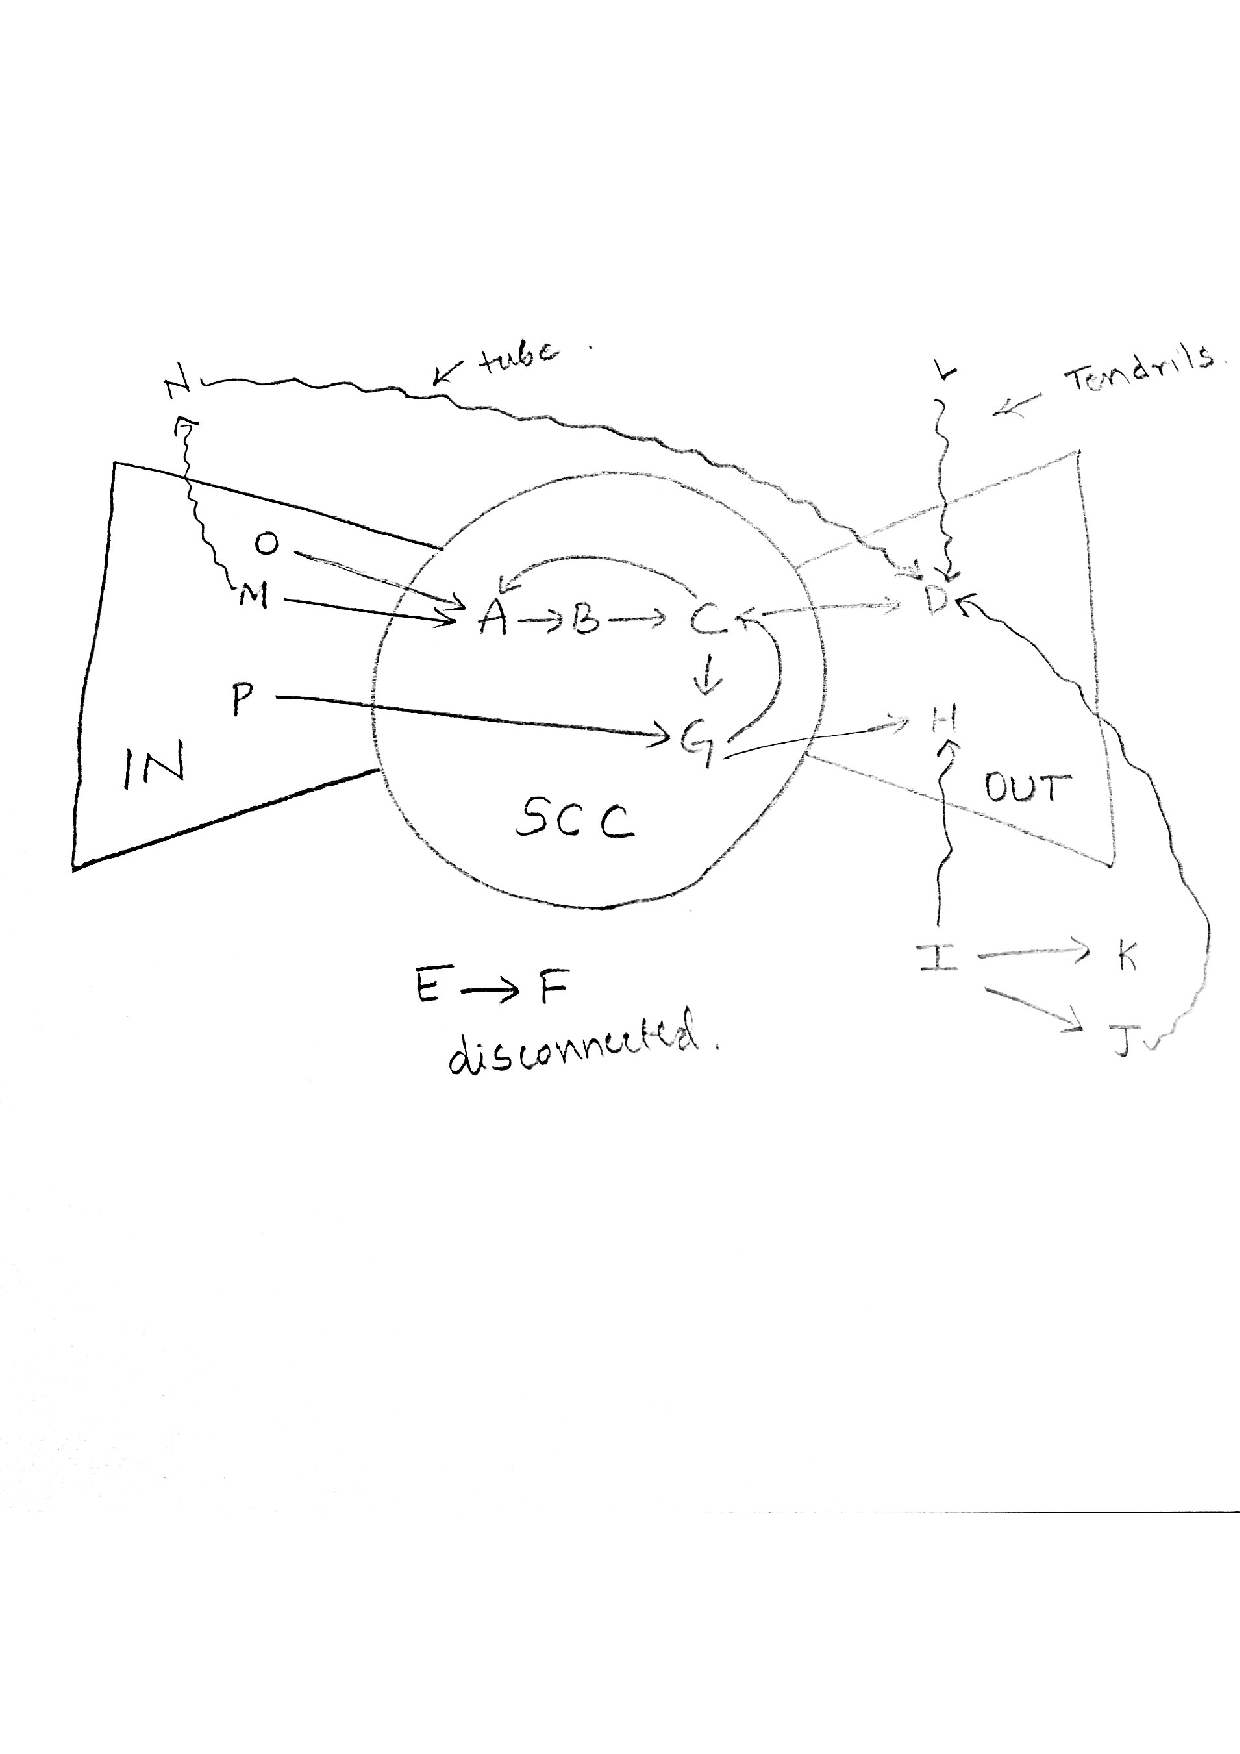
\includepdf[pages={1}]{figures/3question.pdf}

